\documentclass[letter,10pt, twocolumn]{article}
\usepackage[utf8]{inputenc}
\usepackage{graphicx}
\usepackage[english]{babel} 
%\usepackage{lipsum}
\usepackage{parskip}
\usepackage{multicol}
\usepackage{geometry}
\usepackage{hyperref}
\geometry{
 left=20mm, right=20mm,
 top=20mm, bottom=20mm,
 }
\usepackage[usenames,dvipsnames]{color}
\hypersetup{
  colorlinks,
  citecolor=Violet,
  linkcolor=PineGreen,
  urlcolor=Blue} 
 
\usepackage{abstract}

\setlength{\parindent}{0pt} 
\renewcommand{\abstractnamefont}{\normalfont\Large\bfseries}
\renewcommand{\abstracttextfont}{\normalfont\Huge}
\renewcommand{\thesection}{\Roman{section}} 
\renewcommand{\thesubsection}{\thesection.\Roman{subsection}}


\title{Evaluation of the unbinding kinetics of Mineralocorticoid receptor (MR) steroid agonist aldosterone, cortisol, and progesteron ligands using molecular simulations: MD and MC}

\author{Sebastian Aguilera Novoa}
\date{April 14, 2023}


\begin{document}

%\maketitle

\twocolumn[
  \begin{@twocolumnfalse}
    \maketitle
    \begin{abstract}
    \normalsize
    asdasdasd
    \vspace{20pt}
    \end{abstract}
  \end{@twocolumnfalse}
]

\section{Introduction}

Is wildly known the important role of the mineralocorticoid hormone aldosterone (MR/Aldo) in the cardiovascular system, in particular the effects that have in the kidney which have been intensively studied. Nevertheless, several researches have demonstrated the importance of this hormone in the circulatory system. In fact, this hormone is related to several number of common diseases of high mortality and health cost such as hypertension, stroke, heart failure, chronic kidney diseases, obesity, and diabetes disorders which appears when aldosterone is strongly present. Because the main function of MR/Aldo is the regulation of renal sodium balance as well as biological effects several researches have reported its presence in organs like kidney, heart, blood vessels, adipose tissue, brain, eyes, and skin, Figure \ref{MR_functions}. \cite{book-MR_AS4, MR-as4_importance} 


\begin{figure}[h]
%\centering
\hspace*{-15pt}   
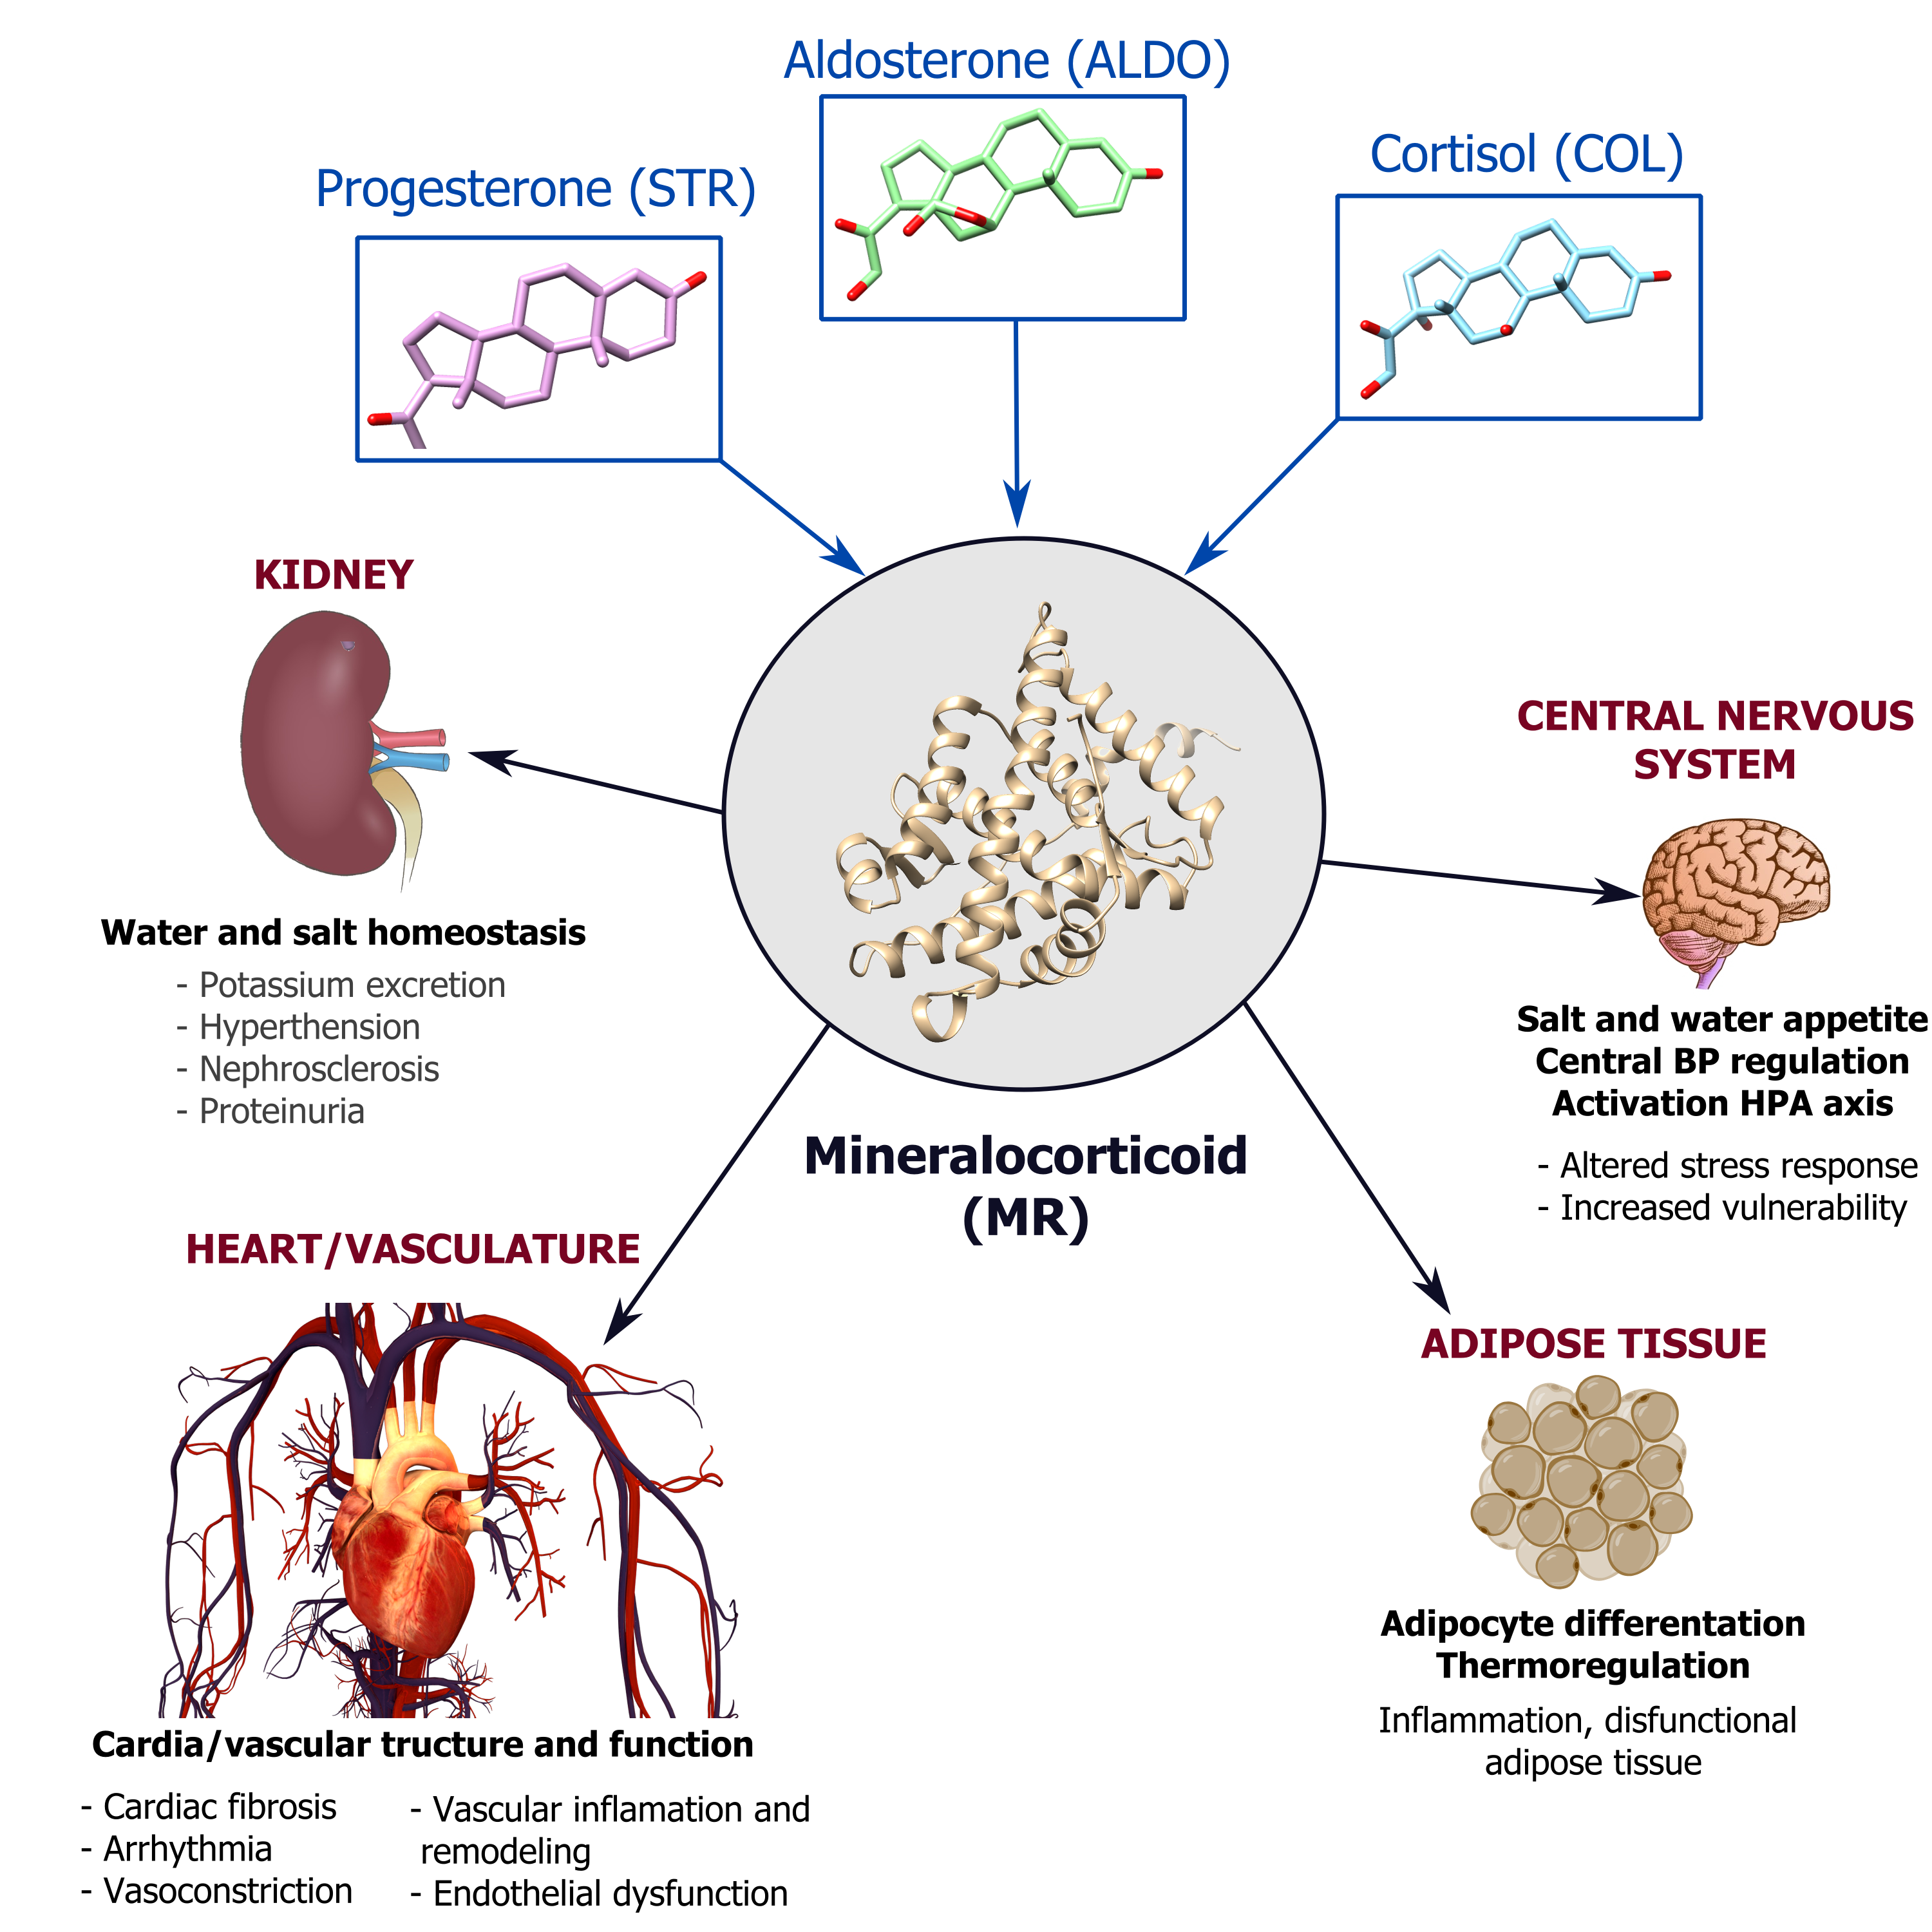
\includegraphics[scale=0.35]{MR-AS4-COL.png}
\caption{Mineralocorticoid/aldosterone receptor impact on health. \textit{Image taken and adapted from \cite{book-MR_AS4}.}}
\label{MR_functions}
\end{figure}

The MR/aldo affinity have been already established, but a discovery at 1987 \cite{discovery}, first studies with recombinant human MR (hMR), showed that hMR has strong binding affinities for several corticosteroids: aldosterone (aldo), cortisol (col), corticosterone, and 11-deoxycorticosterone; and for progesterone (str). \cite{book-MR_AS4} Nowadays is not well known why MR is more sensitive to aldolsterone than to cortisol, this have been showed by ex vivo experiments which also demonstrated that the glucocorticoid cortisol hormone binds to the hMR with the same affinity as aldo, but is less efficient than aldo in stimulating the hMR transactivation. \cite{HELLALLEVY20001250}

Several studies of MR and its mutations have revealed that the substitution of leucine for serine at codon 810 (S810L) in hMR (MR$_{S810L}$) is responsible of early-onset hypertension and pregnancy-related hypertension raising the risk of pre-eclampsia and early hypertension. Clinical studies on hypertensive patients and their families showed that all MR$_{S810L}$ carriers had developed hypertension before they were 20 yr old, whereas who do not present this mutant had normal blood pressure. \cite{Severe, Activating_Mineralocorticoid}

Currently, the crystal structure of MR is known and have been obtained using different methods such as X-Ray Diffraction or Cryogenic Electron Microscopy (CryoEM); even, resent articles have showed the asymmetric dimer form of MR \cite{dimer}. Nevertheless, these methods give just a static view of the protein behavior and do not allow to us to properly describe its dynamical: how MR interacts with a ligand in an un/binding process?. A confident and explored approach to answer this question is the molecular modeling. The huge progress in computational resources has led us to created robust and efficient methods to simulate proteins dynamics, such as Molecular Dynamics (MD) and Monte Carlo (MC) simulations, permitting to the researches explore the dynamics of protein-ligand interactions and given strong explanations to their behavior and are they interacting.  \cite{md_evidence}



orphaz'n question

\section{State of Art}

Selection of the best method to simulate the system, description of the simulation methods and how are we analyzing the date, since the MD simulations have a sense of time while the MC simulations does not, pyEMMA.

Describe how LiGaMD and LiBELa works and the difference between them.


\subsection{Molecular Dynamics (MD)}

\subsubsection*{\textbf{Assisted Model Building with Energy Refinement (Amber)  
}}


\subsubsection*{\textbf{Ligand Gaussian Accelerated Molecular Dynamics 2 (LiGaMD)}}



\cite{amber, ligamd_Miao, ligamd2}

Other option is the \href{https://github.com/pablo-arantes/making-it-rain}{making it rain} project based on LiGaMD and google colab. \cite{making_it_rain}

\subsection{Monte Carlo (MC)}


\subsubsection*{\textbf{Ligand Binding Energy Landscape  (LiBELa)
}}
\cite{libela}

\subsubsection*{\textbf{Python API for Emma's Markov Model Algorithms (PyEMMA)}}


\cite{pyemma}


\section{Methods}





\section{Results and Discussion}

Select images of interest and explain them


\section{Conclusion}


\begin{itemize}

\item LiBELa  is able to reproduce unbinding events in the MR/Aldo-Col-Str systems, even when it simulates just the dynamics of the ligand and consider the protein static.

\item Using LiGaMD is not enough to reproduce un/binding process, no matter how long is the simulation since the electrical potential is strong. 

\item LiGaMD2 is good enough to reproduce un/binding process?

\end{itemize}


\clearpage
\onecolumn{
\bibliography{../references}
\bibliographystyle{unsrt.bst}
%\nocite{*}
}

\end{document}
